\documentclass[11pt]{article}
\usepackage[top=1cm, bottom=2cm, left=1cm, right=1cm]{geometry}
\usepackage{ctex}
\usepackage{float}
\usepackage{algorithm}
\usepackage{algorithmicx}
\usepackage{algpseudocode}
\usepackage{amsthm,amsmath,amssymb}
\usepackage[colorlinks=true,linkcolor=blue]{hyperref}
\usepackage{listings}
\usepackage{xcolor,xparse}
\usepackage{realboxes}
\usepackage{graphics}
\usepackage{graphicx}
\usepackage{mathrsfs}
\usepackage{wrapfig}
\usepackage{subfigure}
\usepackage{pifont}

\definecolor{cmdbg}{rgb}{0.9,0.9,0.9}
\lstset{%
	basicstyle=\ttfamily,
	breaklines = true,
	backgroundcolor=\color{cmdbg},
}
\DeclareDocumentCommand{\ccmd}{v}{% 参数 v 表示工作方法类似于 \verb
    \Colorbox{cmdbg}{\csname lstinline\endcsname!#1!}%
}

\makeatletter
\newenvironment{breakablealgorithm}
  {% \begin{breakablealgorithm}
   \begin{center}
     \refstepcounter{algorithm}% New algorithm
     \hrule height.8pt depth0pt \kern2pt% \@fs@pre for \@fs@ruled
     \renewcommand{\caption}[2][\relax]{% Make a new \caption
       {\raggedright\textbf{\ALG@name~\thealgorithm} ##2\par}%
       \ifx\relax##1\relax % #1 is \relax
         \addcontentsline{loa}{algorithm}{\protect\numberline{\thealgorithm}##2}%
       \else % #1 is not \relax
         \addcontentsline{loa}{algorithm}{\protect\numberline{\thealgorithm}##1}%
       \fi
       \kern2pt\hrule\kern2pt
     }
  }{% \end{breakablealgorithm}
     \kern2pt\hrule\relax% \@fs@post for \@fs@ruled
   \end{center}
  }
\makeatother

\author{李明钰 22307110156}
\title{计算物理作业4}

\begin{document}
\maketitle


\section{题目1:Newton插值法和三次样条插值法}
\subsection{题目描述}
Newton interpolation of:

\begin{itemize}
    \item[1.] 10 equal spacing points of $\cos(x)$ within $[0,\pi]$
    \item[2.] 10 equal spacing points $1/(1+25}x^2)$ within [-1,1].
\end{itemize}

Compare the results with the cubic spline interpolation.


\subsection{程序描述}
先生成十个样本点$x_{1,i} = 0+\frac{\pi}{10} i, y_{1,i} = \cos(x_{1,i})\quad i = 0,1,\ldots 9$然后利用牛顿插值法(算法\ref{Newton插值法})、插值顺序反向后进行牛顿插值法、拉格朗日插值法(算法\ref{Lagrange插值法})、三次样条插值法(算法\ref{Cubic Spline插值法伪代码})分别进行插值,得到插值后的函数$f_{1,NI}$、$f_{1,invNI$、$f_{1,LI}$、$f_{1,CSI}$,并画出函数图像进行对比,然后画出了原函数$f_1 = \cos(x)$减去上述插值得到函数的图像,用以了解各插值方法的误差。

对第二题重复上述操作,但是不再测试插值反向后牛顿插值法的情况。

\subsection{伪代码}
Newton插值法的伪代码如下所示
\begin{breakablealgorithm}
\caption{Newton插值法}
\label{Newton插值法}
\begin{algorithmic}[1]
\State \textbf{Input:} 样本点 $x_{\text{sample}}$ (自变量数组),样本点 $y_{\text{sample}}$ (函数值数组)
\State \textbf{Output:} Newton插值多项式的函数 $P(x)$
\State 设 $n \gets \text{len}(x_{\text{sample}}) - 1$
\State 初始化 $N$ 为零矩阵,大小为 $n \times \text{len}(x_{\text{sample}})$
\State 初始化 $a$ 为零向量,大小为 $n$
\BlankLine
\State \textbf{Step 1:} 计算第一个$a_0$的值
\State $a_0 \gets \frac{y_{\text{sample}, 1} - y_{\text{sample}, 0}}{x_{\text{sample}, 1} - x_{\text{sample}, 0}}$
\State $N_0(x) \gets y_{\text{sample}, 0} + a_0 \cdot (x - x_{\text{sample}, 0})$
\BlankLine
\State \textbf{Step 2:} 迭代计算$a_i$的值 ($i = 1, 2, ..., n-1$)
\For{$i = 1$ \textbf{to} $n-1$}
    \State 设 $N_{\text{part}} \gets 1$
    \For{$j = 0$ \textbf{to} $i$}
        \State $N_{\text{part}} \gets N_{\text{part}} \cdot (x_{\text{sample}} - x_{\text{sample}, j})$
    \EndFor
    \State 计算 $a_i$
    \State $a_i \gets \frac{y_{\text{sample}, i+1} - N_{i-1}(x_{\text{sample}, i+1})}{N_{\text{part}}(x_{\text{sample}, i+1})}$
    \State 更新 $N_i(x)$
    \State $N_i(x) \gets N_{i-1}(x) + a_i \cdot N_{\text{part}}(x)$
\EndFor
\BlankLine
\State \textbf{Step 3:} 定义 Newton 插值多项式函数 $P(x)$
\State $P(x) \gets y_{\text{sample}, 0}$
\For{$i = 0$ \textbf{to} $n-1$}
    \State 设 $y_{\text{part}} \gets 1$
    \For{$j = 0$ \textbf{to} $i$}
        \State $y_{\text{part}} \gets y_{\text{part}} \cdot (x - x_{\text{sample}, j})$
    \EndFor
    \State $P(x) \gets P(x) + a_i \cdot y_{\text{part}}$
\EndFor
\State \Return $P(x)$
\end{algorithmic}
\end{breakablealgorithm}

Lagrange插值法伪代码如下所示
\begin{breakablealgorithm}
\caption{Lagrange插值法}
\label{Lagrange插值法}
    \begin{algorithmic}[1]
\State \textbf{Input:} 样本点 $x_{\text{sample}}$ (自变量数组),样本点 $y_{\text{sample}}$ (函数值数组)
\State \textbf{Output:} Lagrange插值多项式的函数 $P(x)$
\State 设 $n \gets \text{len}(x_{\text{sample}})$
\BlankLine
\Function{A}{$x, j$}
    \State $A \gets 1$
    \For{$i = 0$ \textbf{to} $n-1$}
        \If{$i \neq j$}
            \State $A \gets A \cdot \frac{(x - x_{\text{sample}, i})}{(x_{\text{sample}, j} - x_{\text{sample}, i})}$
        \EndIf
    \EndFor
    \State \Return $A$
\EndFunction
\BlankLine
\Function{LagrangeInterpolatedFunc}{$x$}
    \State $y \gets 0$
    \For{$j = 0$ \textbf{to} $n-1$}
        \State $y \gets y + A(x, j) \cdot y_{\text{sample}, j}$
    \EndFor
    \State \Return $y$
\EndFunction
\BlankLine
\State \Return \Call{LagrangeInterpolatedFunc}{$x$}
\end{algorithmic}
\end{breakablealgorithm}

三次样条插值的伪代码如下所示
\begin{breakablealgorithm}
\caption{Cubic Spline插值法伪代码}
\label{Cubic Spline插值法伪代码}
\begin{algorithmic}[1]
\State \textbf{Input:} 样本点 $x_{\text{sample}}$ (自变量数组),样本点 $y_{\text{sample}}$ (函数值数组)
\State \textbf{Output:} Cubic Spline插值多项式的函数 $P(x)$
\State 设 $n \gets \text{len}(x_{\text{sample}})$
\State 设 $h \gets \text{np.diff}(x_{\text{sample}})$
\State 设 $\delta_y \gets \text{np.diff}(y_{\text{sample}})$
\BlankLine
\State \textbf{Step 1:} 构造三对角矩阵 $A$ 和向量 $b$
\State 初始化 $A$ 为 $n \times n$ 零矩阵
\State 初始化 $b$ 为大小为 $n$ 的零向量
\State 设 $A[0,0] \gets 1$ \Comment{自然边界条件 $S''(x_0) = 0$}
\State 设 $A[n-1,n-1] \gets 1$ \Comment{自然边界条件 $S''(x_n) = 0$}
\For{$i = 1$ \textbf{to} $n-2$}
    \State $A[i, i-1] \gets h[i-1]$
    \State $A[i, i] \gets 2 \cdot (h[i-1] + h[i])$
    \State $A[i, i+1] \gets h[i]$
    \State $b[i] \gets 6 \cdot \left( \frac{\delta_y[i]}{h[i]} - \frac{\delta_y[i-1]}{h[i-1]} \right)$
\EndFor
\BlankLine
\State \textbf{Step 2:} 求解二阶导数向量 $M$
\State 设 $M \gets$ 线性方程组$A\vec{M} = \vec{b}$的解
\BlankLine
\State \textbf{Step 3:} 计算每段的样条系数
\State 初始化 $parameter$ 为 $n-1 \times 4$ 的零矩阵
\For{$i = 0$ \textbf{to} $n-2$}
    \State $parameter[i, 0] \gets y_{\text{sample}, i}$
    \State $parameter[i, 1] \gets \frac{\delta_y[i]}{h[i]} - \frac{h[i]}{6} \cdot (M[i+1] + 2 \cdot M[i])$
    \State $parameter[i, 2] \gets \frac{M[i]}{2}$
    \State $parameter[i, 3] \gets \frac{M[i+1] - M[i]}{6 \cdot h[i]}$
\EndFor
\BlankLine
\Function{CubicSplineInterpolatiedFunc}{$x$}
    \For{$i = 0$ \textbf{to} $n-2$}
        \If{$x_{\text{sample}, i} \leq x \leq x_{\text{sample}, i+1}$}
            \State $y \gets parameter[i,0] + parameter[i,1] \cdot (x - x_{\text{sample}, i})$
            \State $y \gets y + parameter[i,2] \cdot (x - x_{\text{sample}, i})^2$
            \State $y \gets y + parameter[i,3] \cdot (x - x_{\text{sample}, i})^3$
            \State \Return $y$
        \EndIf
    \EndFor
\EndFunction
\BlankLine
\State \Return \Call{CubicSplineInterpolatiedFunc}{$x$}
\end{algorithmic}
\end{breakablealgorithm}
\subsection{运行结果}
运行得到的结果如下图所示,可以发现,对$f_1(x)=\cos(x)$多项式插值效果更好,而对$f_2(x)=\frac{1}{1+25x^2}$样条插值法效果更好。
\begin{figure}[H]
    \centering
    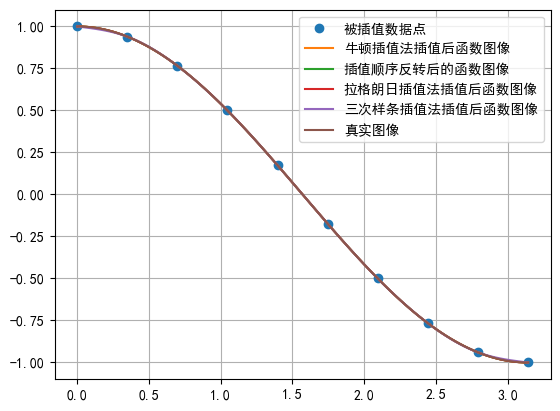
\includegraphics[width=0.5\linewidth]{f1与各插值图像.png}
    \caption{$f_1=\cos(x)$与各插值函数图像}
    \label{fig:$f_1$与各插值得到函数图像}
\end{figure}


\begin{figure}[H]
    \centering
    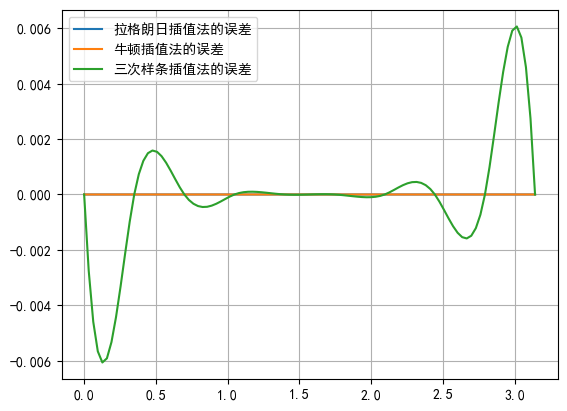
\includegraphics[width=0.5\linewidth]{对f1各插值误差.png}
    \caption{$f_1(x)=\cos(x)$与各插值函数误差}
    \label{fig:f1与各插值函数误差}
\end{figure}

\begin{figure}[H]
    \centering
    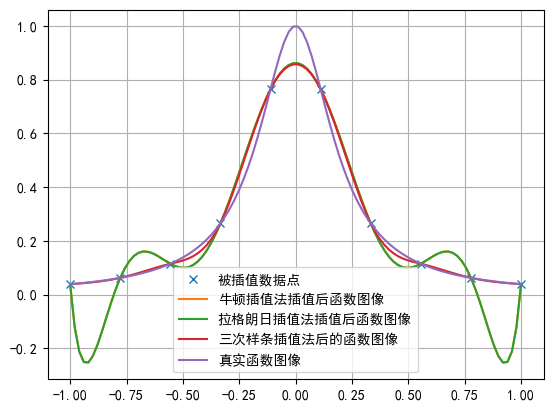
\includegraphics[0.5width=\linewidth]{f2各插值图像.png}
    \caption{$f_2(x)=\frac{1}{1+25x^2}$与各插值函数图像}
    \label{fig:f_2(x)与各插函数图像}
\end{figure}


\begin{figure}[H]
    \centering
    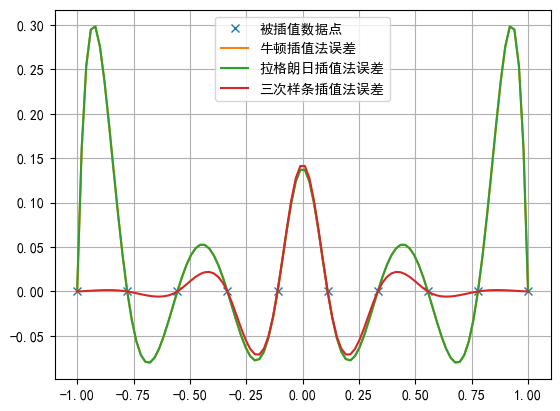
\includegraphics[0.5width=\linewidth]{f2各插值误差.png}
    \caption{$f_2(x)=\frac{1}{1+25x^2}$与各插函数误差}
    \label{f_2(x)与各插函数误差}
\end{figure}

\subsection{附加题证明}
牛顿插值法是根据n+1个点$(x_i,y_i),i=1,2\ldots ,n+1$得到一个n次多项式$P_n(x) = \sum_{i=0}^n a_i x^i$,实际上是一个解(n+1)元线性方程组的过程,事实上,过这n+1个点的n次多项式只有一个形式,因此不管如何改变牛顿插值法的插入顺序其结果都相同且与拉格朗日插值法得到结果相等。

这一结果也可以由对$f_1(x)$的插值结果验证
\begin{figure}[H]
    \centering
    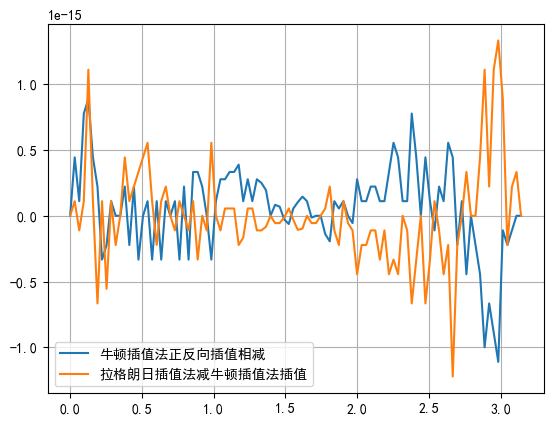
\includegraphics[width=0.5\linewidth]{多项式插值相减.png}
    \caption{多项式插值相减.png}
    \label{fig:my_label}
\end{figure}

\section{题目2:线性拟合与抛物线拟合}
\subsection{题目描述}
The table below gives the temperature $T$ along a metal rod whose ends are kept at fixed constant temperatures. The temperature is a function of the distance $x$ along the rod. 

\begin{array}{c|ccccccccc}\hline x_i\left(\text{cm}\right)&1.0&2.0&3.0&4.0&5.0&6.0&7.0&8.0&9.0\\T_i\left(\text{°C}\right)&14.6&18.5&36.6&30.8&59.2&60.1&62.2&79.4&99.9\\\hline\end{array}

\begin{itemize}
    \item[1.] Compute a least-squares, straight-line fit to these data using $T(x)=ax+b$
    \item[2.] Compute a least-squares, parabolic-line fit to these data using $T(x) = a+bx+cx^2$
\end{itemize}
\subsection{程序描述}
利用线性和最小二乘法,分别计算除了线性拟合和抛物线拟合的结果,并计算出来相应的$R^2$。
\subsection{伪代码}
\begin{breakablealgorithm}
    \caption{Straight Line Fit}
    \begin{algorithmic}[1]
        \Function{StraightLineFit}{x, y}
            \State $n \gets \text{len}(x)$
            \State $a \gets \frac{\sum (x \cdot y) - n \cdot \text{mean}(y) \cdot \text{mean}(x)}{\sum (x^2) - n \cdot (\text{mean}(x))^2}$
            \State $b \gets \text{mean}(y) - a \cdot \text{mean}(x)$
            \State \Return $a, b$
        \EndFunction
    \end{algorithmic}
\end{breakablealgorithm}
\begin{breakablealgorithm}
    \caption{Parabolic Line Fit}
    \begin{algorithmic}[1]
        \Function{ParabolicLineFit}{x, y}
            \State $n \gets \text{len}(x)$
            \State $X \gets \text{zeros}(n, 3)$
            \For{$i = 0$ \textbf{to} $n-1$}
                \For{$j = 0$ \textbf{to} $2$}
                    \State $X[i][j] \gets x[i]^j$
                \EndFor
            \EndFor
            \State $a \gets (\text{inv}(X^T \cdot X) \cdot (X^T \cdot y))$
            \State \Return $a[0], a[1], a[2]$
        \EndFunction
    \end{algorithmic}
\end{breakablealgorithm}
\subsection{运行结果}
\begin{figure}[H]
    \centering
    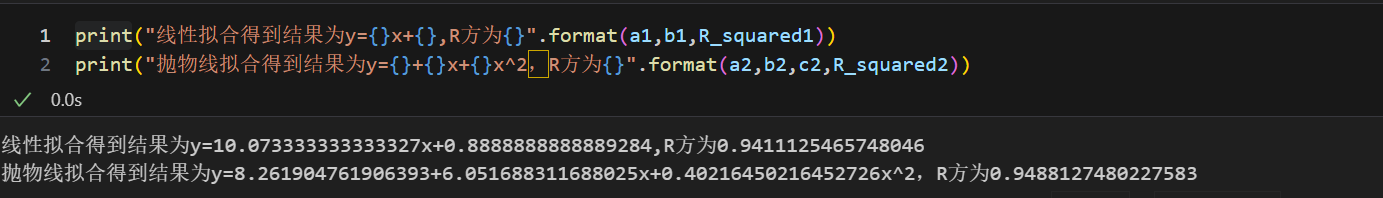
\includegraphics[width=0.5\linewidth]{拟合结果.png}
    \caption{拟合结果}
    \label{fig:拟合结果}
\end{figure}

\begin{figure}[H]
    \centering
    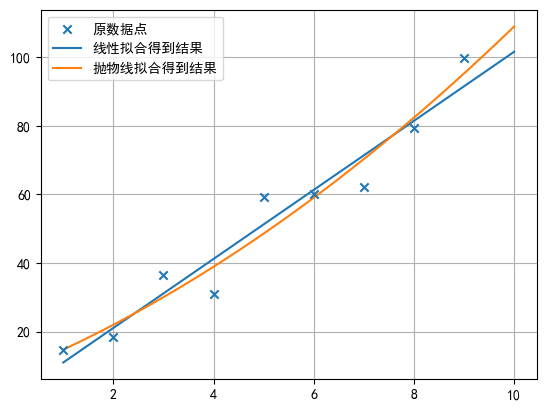
\includegraphics[width=0.5\linewidth]{拟合图像.png}
    \caption{拟合图像}
    \label{fig:拟合图像}
\end{figure}
\end{document}
